\documentclass[../main]{subfiles}
\begin{document}

\section{Qualità del software}
La \g{qualità} in un progetto software ha diversi destinatari e quindi diversi scopi. È un aspetto imprescindibile in un \g{progetto software} professionale, talmente tanto che non è un fattore tipicamente indicato come requisito, perché implicito e preteso da tutti. La \g{qualità} del \g{prodotto software} interessa a chi:
\begin{itemize}
    \item Crea il prodotto (il fornitore), che deve essere conforme ai requisiti e idoneo all'uso, anche per sapere come si pone rispetto ai suoi competitor;
    \item Usa il prodotto (il committente o cliente), che deve essere soddisfatto;
    \item Valuta il prodotto (in maniera sistematica), che deve poter misurare le caratteristiche di qualità.
\end{itemize}
Il controllo di \g{qualità} deve essere costante (ma come si è sempre detto non preponderante e non bloccante) e non tardivo, poiché va fatto durante lo sviluppo. Deve esserci un \g{sistema di qualità}.
\subsection{Sistema di qualità}
Il \g{sistema di qualità} deve essere parte del ciclo di miglioramento continuo nello sviluppo, nel \g{controllo di qualità} (\textit{come fare per produrre qualità}) e nel \g{piano di qualità} (\textit{cosa fare per avere qualità}).
Il \g{piano di qualità}, per garantire di essere sistematici, disciplinati e quantificabili, richiede che il fornitore:
\begin{itemize}
    \item Fissi delle politiche per il perseguimento della qualità;
    \item Determini gli obiettivi di qualità;
    \item Usi procedure e strumenti ritenuti \g{best practice}.
\end{itemize}
Il \g{controllo di qualità} è ciò che viene svolto per verificare il rispetto di quanto dichiarato nel piano di qualità. Esso è preferibile sia \textit{preventivo} e non \textit{retrospettivo}, per assicurare il rispetto del \g{piano di qualità}. Ecco perché è più probabile imbattersi nel termine \textit{Quality Assurance} (accertamento di qualità) più spesso che in controllo.
\subsection{Standard di qualità}
Uno standard è un documento, tipicamente redatto da un ente internazionale, che forma una raccolta organica (ovvero di elementi che si completano a vicenda per uno scopo finale, in questo caso la qualità) di \g{best practice}.
Adottare uno standard, o assumerlo come fonte informativa, è utile perché permette di adeguarsi all'uso di \g{best practice} consolidate. La sua adozione e integrazione nel \g{way of working} di \g{progetto} permette di evitare errori già fatti in passato (anche da altri) e di mettere in atto nel proprio ciclo di miglioramento continuo la Quality Assurance.
Bisogna però stare attenti a cercare di recepire uno standard mediante l'uso di strumenti informatici o il rispetto di certe norme rischia di diventare frustrante e il team del progetto o aziendale evita di metterlo in pratica per evitare la perdita di tempo richiesta da eccessiva burocrazia.
\subsection{Modello di standard}
Gli standard sono realizzati in modo da poter facilitare la valutazione della loro adozione:
\begin{itemize}
    \item Rispetto all'uso da parte dell'utente;
    \item Rispetto alla produzione da parte del fornitore;
    \item Rispetto al rapporto costi/benefici.
\end{itemize}
Tutto ciò in un modello unico per tutti i destinatari.
Alcuni standard di qualità sono:
\begin{itemize}
    \item ISO/IEC 9126:2001 \textit{SWE Product Quality}, definisce le caratteristiche di qualità rilevanti in un \g{prodotto software};
    \item ISO/IEC 14598:1999 \textit{SW Product Evaluation}, definisce metriche di valutazione in base al destinatario (fornitore, committente, valutatore);
    \item ISO/IEC 25000:2005 \textit{Systems and software Quality Requirements and Evaluation (SQuaRE)}, riunisce in un unico documento lo standard 9126 e il 14598.
\end{itemize}
Della serie di standard 25000 ne sono state prodotte altre versioni, riassunte nella seguente immagine:
\begin{figure}[h]
    \begin{center}
        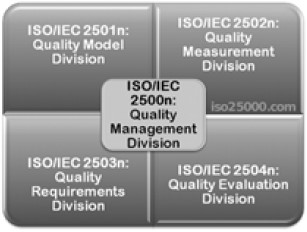
\includegraphics[scale=0.8]{immagini/iso25000.jpg}
    \end{center}
\end{figure}
Le caratteristiche di qualità un prodotto devono essere misurabili e questo significa che deve essere possibile assegnare un valore numerico o preso da una scala di valori (un valore oggettivo, non soggettivo) a ciascuna delle caratteristiche definite per il prodotto.
Alcuni esempi di metriche di qualità per un \g{prodotto software} sono: Source Line Of Code (SLOC), relativamente al codice sorgente; person/days, per valutare il lavoro da impiegare, l'indice di Gunning Fog, per il testo.
\end{document}